% ****** Start of file apssamp.tex ******
%
%   This file is part of the APS files in the REVTeX 4.1 distribution.
%   Version 4.1r of REVTeX, August 2010
%
%   Copyright (c) 2009, 2010 The American Physical Society.
%
%   See the REVTeX 4 README file for restrictions and more information.
%
% TeX'ing this file requires that you have AMS-LaTeX 2.0 installed
% as well as the rest of the prerequisites for REVTeX 4.1
%
% See the REVTeX 4 README file
% It also requires running BibTeX. The commands are as follows:
%
%  1)  latex apssamp.tex
%  2)  bibtex apssamp
%  3)  latex apssamp.tex
%  4)  latex apssamp.tex
%
\documentclass[%
 reprint,
%superscriptaddress,
%groupedaddress,
%unsortedaddress,
%runinaddress,
%frontmatterverbose, 
%preprint,
%showpacs,preprintnumbers,
%nofootinbib,
%nobibnotes,
%bibnotes,
 amsmath,amssymb,
 aps,
%pra,
%prb,
%rmp,
%prstab,
%prstper,
%floatfix,
]{revtex4-1}

\usepackage{graphicx}% Include figure files
\usepackage[utf8]{inputenc}
\usepackage{dcolumn}% Align table columns on decimal point
\usepackage{bm}% bold math
%\usepackage{hyperref}% add hypertext capabilities
%\usepackage[mathlines]{lineno}% Enable numbering of text and display math
%\linenumbers\relax % Commence numbering lines

%\usepackage[showframe,%Uncomment any one of the following lines to test 
%%scale=0.7, marginratio={1:1, 2:3}, ignoreall,% default settings
%%text={7in,10in},centering,
%%margin=1.5in,
%%total={6.5in,8.75in}, top=1.2in, left=0.9in, includefoot,
%%height=10in,a5paper,hmargin={3cm,0.8in},
%]{geometry}

\begin{document}

\preprint{APS/123-QED}

\title{Osciloscopio}% Force line breaks with \\
\thanks{}%

\author{Jesus Prada}
 \email{jd.prada1760@uniandes.edu.co}
 \altaffiliation[Also at ]{Departamento de Física, Universidad de los Andes}%Lines break automatically or can be forced with \\
\author{Sergio Iv\'an Rey}%
 \email{si.rey1826@uniandes.edu.co}
\affiliation{%
 Departamento de Física, Universidad de los Andes
}%

\date{13/8/2015}% It is always \today, today,
             %  but any date may be explicitly specified

\begin{abstract}
Durante la presente práctica se estudiaron los fen\'omenos ondulatororios en circuitos RC, RLC y en osciladores perpendiculares. En una primera instancia se determin\'o experimentalmente el tiempo de caracter\'istico de carga y descarga de un condensador. Donde se encontró $\tau = 274 \pm 4ms$ para la configuración $ R = 470\Omega, C = 470\mu F$  y $\tau = 478 \pm4\mu s$ para la configuración $ R = 470\Omega, C = 47\mu F$. Estas medidas tienen un error del 25\%  y del 1\% respectivamente. Esto, y otros argumentos presentados nos llevaron a pensar que en la primera configuración los dispositivos usados estaban en mal estado. En segunda instancia, se construy\'o un circuito RLC en serie  con $C=47nF, L = 2mH, R= 0.8\Omega$, donde se midió la frecuencia natural del sistema $f_0 = \frac{1}{2\pi\sqrt{LC}}$, y por dos m\'etodos diferentes se determin\'o el parámetro de resistencia $\gamma = \frac{R}{L}$. Los resultados obtenidos fueron $f_0 =  16.583 \pm 0.03KHz$, lo cual tiene un error de 1\% respecto a su valor teórico, y $\gamma = 25.639 \pm 0.4 KHz $, lo cual tiene un error muy alto pero consistente con dos experimentos, por lo que se deduce que se subestimó la resistencia del circuito general. Para los osciladores perpendiculares se confirmaron cualitativamente varios aspectos teóricos de las curvas que formaban.\\
\end{abstract}


\keywords{Oscilaciones forzadas, Oscilaciones Amortiguadas, RC, RLC}%Use showkeys class option if keyword
                              %display desired
\maketitle

%\tableofcontents

\section{\label{sec:level1}Introducci\'on}

Las resistencias, capacitancias e inductancias son de los componentes m\'as fundamentales de los circuitos electr\'onicos. Su comportamiento puede ser cuantificado con gran exactitud y por esta raz\'on sirven para estudiar diversos sistemas que van desde sistemas no oscilatorios hasta sistemas de oscilaciones forzadas y amortiguadas. Las diversas aplicaciones de los circuitos RC, RL, LC, RLC, etc. van desde transformadores AC a DC, filtros de señales, hasta generadores simples de voltaje. Estos circuitos son los componentes primordiales de elementos cotidianos como las buj\'ias, los flashes de c\'amaras fotogr\'aficas, etc.\\

En primera instancia, en este laboratorio nos interesamos en estudiar el proceso de carga y descarga de un capacitor en un circuito RC en serie bajo una diferencia de potencial constante ($V_f$). Si se obtiene la ecuación diferencial para la carga del capacitor en estos sistemas, es sencillo demostrar que las funciones de voltaje sobre la resistencia para el sistema de carga ($V_c$) y descarga ($V_d$) son respectivamente:\\

\begin{equation}
Vc(t) = V_fe^{-t/{RC}}
\end{equation}
\begin{equation}
Vd(t) = -V_fe^{-t/{RC}}
\end{equation}

En estas ecuaciones, $\tau = RC$ es una constante fundamental que indica qu\'e tan r\'apido se carga o descarga el capacitor. Esta constante indica en cu\'anto tiempo el voltaje en la resistencia llega a un factor de $e^{-1} \approx 37\% $ de su valor inicial. \\

En segunda instancia, para caracterizar un sistema oscilatorio forzado y amortiguado con el osciloscopio, nos propusimos estudiar un circuito RLC en serie. Para este tipo de circuitos, la ecuaci\'on diferencial que caracteriza la carga almacenada en el capacitor es lineal de segundo orden. De forma general, la ecuación diferencial este tipo de sistemas es de la forma:\\

\begin{equation}
\frac{d^2q}{dt^2} + \gamma\frac{dq}{dt} + \omega_0^2q = \frac{F_0}{m}e^{i\omega t}
\end{equation}

Aqu\'i $\omega$ es la frecuencia de forzamiento de la fuente y $F_0$ su amplitud. El par\'ametro $m$ ser\'ia la masa en un sistema mec\'anico. $\omega_0$ es la frecuencia natural del sistema. El par\'ametro $\gamma$ hace referencia a la perdida de energ\'ia del sistema, por fricci\'on en sistemas mec\'anicos, y por resistencia en los electr\'onicos. Estos dos \'ultimos par\'ametros determinan la resonancia del sistema respecto a la fuente de forzamiento, e incluso determinan si la ecuaci\'on diferencial acepta o no soluciones oscilatorias en el caso en que no haya forzamiento ($\omega = 0$).\\

Sin mucho esfuerzo, analizando el circuito RLC en s\'i, es posible deducir que $m \equiv L$, $F_0 \equiv V_f$ y que los valores de los par\'ametros de frecuencia y fricci\'on están dados por: \cite{ondas}\\

\begin{equation}
\omega_0 = \frac{1}{\sqrt{LC}}
\end{equation}
\begin{equation}
\gamma = R/L
\end{equation}

Si hay la fuente es una onda sinusoidal, es decir, si hay forzamiento, la ecuaci\'on diferencial solo aceptar\'a soluciones de tipo sinusoidal, con frecuencia igual a la de forzamiento ($q(t) = Ae^{i\omega + \delta}$) . En este caso, lo importante es analizar la amplitud de las soliciones en t\'erminos de la frecuencia de forzamiento. Si insertamos la soluci\'on propuesta en la ecuaci\'on diferencial, obtenemos una expresi\'on para la amplitud del sistema en t\'ermonos de la frecuencia de forzamiento: \cite{ondas}

\begin{equation}
A(\omega) = \frac{V_f/L}{\sqrt{(\omega^2 - \omega_0^2)^2 + (\gamma\omega)^2}}
\label{equation:amplitud}
\end{equation}

Derivando esta expresi\'on, se puede encontrar la frecuencia de forzamiento ($\omega_m$) que produce el m\'aximo de amplitud en el sistema. \'Esta frecuencia estar\'a dada por:\\

\begin{equation}
\omega = \sqrt{\omega_0^2 - \frac{\gamma^2}{2} }
\end{equation}

De la misma manera es sencillo demostrar que el ancho de la curva de resonancia, es decir, la distancia entre los dos valores de frecuencia que producen la mitad de la amplitud m\'axima, est\'a dado por:\\

\begin{equation}
\Delta\omega = \frac{1}{\tau} = \gamma = \frac{R}{L}
\end{equation}

En tercera instancia, para analizar un sistema no forzado y amortiguado, tomamos el mismo circuito RLC, esta vez, bajo una fuente directa. En este caso, si se tiene una resistencia lo suficientemente pequeña, la ecuaci\'on diferencial admitir\'a soluciones oscilatorias. En dicho caso, la solución a la ecuaci\'on diferencial (3), con $\omega = 0$  es una onda con la frecuencia $\omega_a = \sqrt{\omega_0^2 -\frac{\gamma^2}{4}}$ , con amplitud modulada por una exponencial determinada por la resistencia. Esta soluci\'on se presenta de la siguiente manera: \cite{ondas}\\

\begin{equation}
V(t) = V_0 e^{\frac{-\gamma t}{2}}\cos(\omega_a t + \delta)
\label{equation:amortiguado}
\end{equation}

Por otra parte, los sistemas electrónicos son generalmente más precisos que los sistemas mecánicos, por lo que si se tiene a la mano un osciloscopio y varios generadores de señales, se puede analizar cualitativamente varios aspectos de los sistemas oscilatorios. Un ejemplo de análisis cualitativo que se puede hacer con estos elementos son las curvas de Lissajous. Estas curvas consisten en la superposición de dos movimientos armónicos simples con distintos parámetros de frecuencia y amplitud. De la forma más general, las figuras de Lissajous son determinadas curvas paramétricas del siguiente estilo:\\


\begin{align*}
x(t) = A_x \cos{(\omega_x t )}\\
y(t) = A_y \cos{(\omega_y t + \delta)}
\end{align*}

Si ambas param\'etricas tienen la misma frecuencia $\omega$ y un desfase $\delta$ nulo, tendremos el caso de una recta de la forma $ y = \frac{A_y}{A_x}x $. Por otra parte, si su desfasaje es igual a $\frac{pi}{2}$, es sencillo demostrar que la curva que se describe es una elipse de tipo $ (\frac{y}{A_y})^2 + (\frac{y}{A_y})^2 = 1 $. Si las frecuencias no son las mismas, las figuras de Lissajous se vuelven complicadas y difíciles de analizar con herramientas simples. Aún así, se puede afirmar que las curvas de serán cerradas siempre que las frecuencias sean conmesurables.



\section{\label{sec:level1}Montaje experimental}
El equipo que se utiliz\'o durante la práctica consist\'ia de dos generadores de onda, un osciloscopio, capacitores, inductores y resistencias de diferentes valores.\\

Para el primer montaje, se configur\'o el generador de onda para que generara una onda cuadrada con una frecuencia de 10Hz y una aplitud de 10V, sin embargo la sonda que conctaba \'este al osciloscopio distorsionaba los valores le\'idos. El circuito montado es un circuito RC en serie como el que se muestra en la figura.\\

\begin{figure}[h!]
\caption{Montaje de Circuito RC en Serie}
\centering
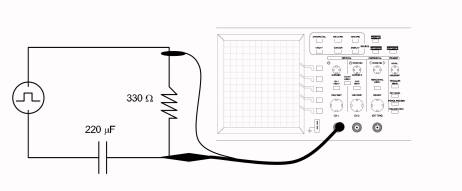
\includegraphics[width=0.45\textwidth]{rc}
\end{figure}

Para la segunda manipulaci\'on, el generador de onda se reajust\'o para generar una onda sinusoidal, a continuaci\'on se construy\'o un circuito RLC en serie como el que se muestra en la figura. En este caso, el valor de R lo proporciona el inductor mismo. Luego, teniendo montado el mismo circuito, se cambi\'o la forma de la señal a onda cuadrada. Debe anotarse que los valores de las figuras no son necesariamente los usados durante la pr\'actica. \\

\begin{figure}[h!]
\caption{Montaje de Circuito RLC en Serie}
\centering
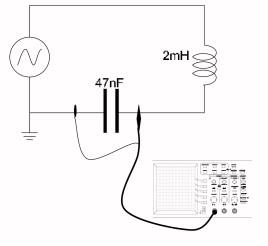
\includegraphics[width=0.30\textwidth]{rlc}
\end{figure}


La tercera manipulaci\'on, consisti\'o en conectar ambos generadores de onda directamente al osciloscopio para simular dos osciladores acoplados y ver el fen\'omeno de las Figuras de Lissajous. Ambos estaban ajustados para generar ondas sinusoidales. El ajuste posterior requiri\'o solamente de la calibraci\'on del osciloscopio para mostrar una señal como funci\'on de la otra. 


\section{\label{sec:level1}Resultados y An\'alisis}

\subsection{\label{sec:level2}Circuito RC en serie}
Para esta manipulaci\'on se utilizaron dos combinaciones de resistencia y capacitor. En primer lugar, $R = 470\Omega$ y $C=470\mu F$ y en segundo lugar, $R=10K\Omega$ y $C = 47nF$. Para la primera configuraci\'on el generador de onda se ajust\'o para generar una onda cuadrada, de tal manera que se pudiera simular un impulso de corriente directa. Dado que el valor nominal esperado de $\tau$ era de 22ms, se ajust\'o la frecuencia del circuito a 5Hz para que en cada pico se pudiera apreciar significativamente el decaimiento del voltaje en el sistema.\\

Se procedi\'o a medir $\tau$ buscando un valor en la curva de decaimiento que correspondiera al 37\% del valor m\'aximo de voltaje alcanzdo que era de $V_max=155\pm 1V$. Su 37\% correspondiente es de 57.35V, que, por cuestiones de resoluci\'on s\'olo se pudo llegar a medir 57V. Para la configuración $R=10K\Omega$ y $C = 47nF$ se hizo el mismo procedimiento. Los datos obtenidos se consignaron en la tabla I.\\

\begin{table}[h!]
\centering
\begin{tabular}{|c|c|c|c|}
\hline
$C$ (F) & $R$ ($\Omega$) & $\tau$ (ms) & Proceso\\
\hline
470$\times 10^{-6}$ & 470 & 276 & Carga\\
470$\times 10^{-6}$ & 470 & 272 & Descarga\\
47$\times 10^{-9}$ & 10000 & 0.480 & Carga\\
47$\times 10^{-9}$ & 10000 & 0.476 & Descarga\\
\hline
\end{tabular}
\caption{Tiempos de carga y descarga, circuito RC en serie}
\end{table}

La mínima resolución medida en tiempo era de aproximadadmente 4ms para la primera configuración y 4$\mu$s para la segunda configuración. Entre las configuraciones solo se cambió la escala del tiempo. Si tomamos el valor promedio en cada medida, los resultados de este experimento fueron $\tau = 274 \pm 4ms$ para el primer experimento y $\tau = 478 \pm 4\mu s$ para la  segunda configuración. Los errores porcentuales fueron del  25\% y del 1\% respectivamente. \\

Cabe resaltar que en un principio la segunda configuración (diferente a la aquí presentada) daba un error del 300\% y daba un valor de capacitancia que era dos órdenes de magnitud alejados de la realidad. En los experimentos RLC se midió este mismo valor de capacitancia por lo que se concluyó que la capacitancia usada estaba desgastada. Decidimos repetir el experimento con la segunda configuración con distintas resistencias y capacitancias y obtuvimos los valores presentados acá. Esto nos sirve para justificar que el error del 25\% obtenido con la primera configuración puede deberse, además de la inexactitud de la medida y el uso de aproximación para $37\% V_0$, al desgaste de las resistencias y capacitancias.\\


\subsection{\label{sec:level2}Circuito RLC Forzado}
En este montaje utilizamos los valores $R = 0.8\Omega$, $L = 2mH$ y $C = 47nF$. Como se puede inferir, decidimos tomar \'unicamente la resistencia del inductor y dem\'as componentes del circuito. Con esta configuraci\'on pod\'iamos apreciar mejor la curva de resonancia y determinar mejor su m\'aximo. Una vez identificado el m\'aximo de amplitud, tomamos 16 datos de frecuencia y voltaje (pp y rms) alrededor del m\'aximo. Dichos datos se presentan en la tabla \ref{table:resonancia}. \\

En estos resultados, la precisi\'on de la frecuencia por medio del generador era enorme, por lo que no la tendremos en cuenta. En este experimento trabajamos con frecuencias del orden de $10kHz$ y el generador permit\'ia cambiar la frecuencia hasta el orden de los $mHz$. Por su parte, la precisi\'on del voltaje estaba dada por el osciloscopio, el cual mostraba usualmente 3 cifras significativas. En general, el error asociado a las mediciones de voltaje se deb\'ia a la inestabilidad de la medida y no a la restricci\'on por cifras significativas. El osciloscopio mostraba valores cercanos que variaban mientras el sistema estaba en una sola configuraci\'on. Los valores de voltaje fueron tomados en donde el osciloscopio se mostraba por m\'as tiempo. El error asociado a todas las medidas de voltaje en este montaje, lo tomamos $0.3V$, ya que ese era el rango en el que variaban los voltajes mostrados para una sola configuraci\'on.\\

Por otra parte, para una señal sinusoidal, los valores $V_{pp}$ y $V_{rms}$ est\'an relacionados por un factor de $\sqrt{2}$. Por lo tanto, usar uno u otro para el an\'alisis es equivalente. Sin embargo, el valor $V{pp}$ presenta menor error relativo al ser m\'as grande, por lo que decidimos hacer el an\'alisis cuantitativo con dichas cantidades.\\

\begin{table}[h!]
\centering
 \begin{tabular}{|c|c|c|} 
 \hline
 $Frecuencia$ (Hz) & $V_{pp}$ (V) & $V_{rms}$ (V) \\ [0.5ex] 
 \hline\hline
16.3 &		12.6 &		4.37\\
16.5 &		12.5 &		4.35\\
16.7 &		12.4 &		4.3\\
17.0 &		12 &		4.18\\
17.5 &		11.1 &		3.85\\
18.0 &		9.84 &		3.41\\
16.1 &		12.5 &		4.36\\
16.9 &		12.4 &		4.3\\
15.6 &		12 &		4.16\\
15.2 &		11.4 &		3.93\\
14.5 &		10 &		3.42\\
14.0 &		9.28 &		3.19\\
13.0 &		7.84 &		2.72\\
12.0 &		6.96 &		2.37\\
19.0 &		7.60 &		2.62\\
20.0 &		5.76 &		1.98\\
[1ex] 
 \hline
 \end{tabular}
 \caption{Datos de curva de resonancia RLC.}
 \label{table:resonancia}
\end{table}

Para obtener el máximo de resonancia de la curva dada por la tabla \ref{table:resonancia}, realizamos computacionalmente un ajuste de parámetros de dichos datos (con $V_{pp}$) teniendo en cuenta que te\'oricamente deber\'ian tener la forma de la ecuaci\'on \ref{equation:amplitud}. Dicho ajuste de parámetros itera de manera no aleatoria sobre los par\'ametros a ajustar decidiendo cual configuraci\'on produce la curva m\'as cercana a los datos. Los par\'ametros ajustados fueron la frecuencia natural $\omega_0$ del sistema, el par\'ametro $\gamma$ de resistencia, y la amplitud $V_f/L$ por la que no nos interesaremos. Este m\'etodo computacional hace parte de la librer\'ia Optimization de ScyPy y permite adem\'as estimar el rango de error de los par\'ametros ajustados. Los resultados gr\'aficos y cuantitativos del ajuste est\'an presentes en la figura \ref{fig:resonancia}.\\

\begin{figure}[h]
\caption{Ajuste de parámetros para la curva de resonancia}
\centering
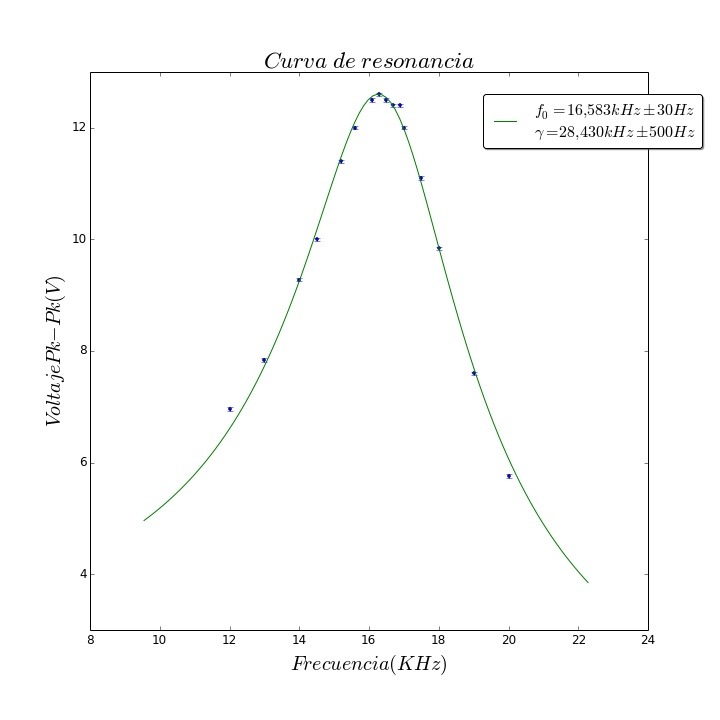
\includegraphics[width=0.45\textwidth]{resonancia}
\label{fig:resonancia}
\end{figure}

En esta gráfica se puede ver que el ajuste fue bastante preciso. Para verificarlo, tomamos el valor real de frecuencia angular natural $f_0^{Teo} = \frac{1}{2\pi \sqrt{LC}} = 1.,416kHz$ y lo comparamos con el valor experimental obtenido  $f_0^{Exp} = 16.583kHz$. Debido a que no teníamos el error teórico, no sabremos con exactitud si el valor experimental entra en el rango aceptado. A pesar de esto, podemos afirmar que el error absoluto asociado a esta medición es del $1\%$.\\

De la misma manera podemos calcular experimentalmente el valor del t\'ermino $\gamma$ de resistencia. En teoría, dicho valor, teniendo en cuenta un\'icamente el valor de resistencia aportado por la inductancia, est\'a dado por $\gamma^{Teo} = \frac{R}{L} = 400Hz$; experimentalmente, esta cantidad tiene un valor de $\gamma^{Exp} = 28.430KHz$. Estos valores están desfasados por casi 2 \'ordenes de magnitud probablemente por no tener en cuenta todos los valores de resistencia asociados a los dem\'as aparatos usados.\\

Adem\'as del m\'etodo anterior podemos confirmar esta medida calculando el ancho de banda de la curva de resonancia. Teniendo el ajuste de par\'ametros, tenemos la funci\'on en pr\'acticamente cualquier frecuencia deseada. Con esto es muy sencillo calcular num\'ericamente y con gran precisi\'on el m\'aximo real de la curva. Con este m\'aximo, que se encuentra en $16,270KHz$ (se encuentra antes de la frecuencia natural como es esperado) podemos calcular los el valor que se tiene que alcanzar para calcular el ancho de banda ($\frac{A_{max}}{\sqrt{2}}$). Una vez calculados los valores de frecuencia que lo cumplen, obtenemos su diferencia y eso nos da el ancho de banda. El valor experimental obtenido para el ancho de banda es en este caso $\gamma^{ExpBW} = 28,996KHz$, lo cual confirma nuestro resultado anterior y le da fuerza a nuestro argumento. Podr\'iamos obtener $\gamma$ otra vez comparando la frecuencia angular natural $\omega_0$ y la frecuencia que provoca el m\'aximo en la curva de resonancia, sin embargo, este m\'etodo ser\'ia redundancia del ancho de banda y del uso de par\'ametros ajustados.\\
 

\subsection{\label{sec:level2}Circuito RLC Amortiguado}
En este montaje, el \'unico aspecto que variamos con respecto al anterior fue la forma funcional de la fuente, es decir, los valores de R, L y C se mantuvieron constantes. En el circuito RLC forzado usamos una fuente sinusoidal que provocaba el forzamiento, mientras que en el montaje RLC amortiguado usamos una fuente cuadrada peri\'odica. \'Esta se comporta como corriente directa por la mitad del periodo y luego cambia instant\'aneamente el signo del voltaje aplicado, manteniendo la señal directa. Si analizamos el circuito en los intervalos de tiempo en que se comporta como con corriente directa, analizamos un circuito RLC amortiguado.\\ 

En este experimento pretend\'iamos obtener el par\'ametro $\gamma$, para lo cual solo era necesario obtener la envolvente, es decir los puntos m\'aximos y m\'inimos de la curva de voltaje contra tiempo. Debido al amortiguamiento de la señal, solo se pudieron tomar 9 datos en el intervalo de corriente directa. Estos datos est\'an consignados en la tabla \ref{table:amortiguado}.\\

\begin{table}[h!]
\centering
 \begin{tabular}{|c|c|} 
 \hline
 $V$ (V) & $t\ (\mu s)$ \\ [0.5ex] 
 \hline\hline
9.2&	20\\
4.4&	80\\
2.2&	140\\
1.0&	200\\
0.6&	262\\
-6.0&	50\\
-2.6&	110\\
-1.2&	170\\
-0.6&	230\\
9.2 & $\infty$ \\
[1ex] 
 \hline
 \end{tabular}
 \caption{Datos de señal RLC amortiguado.}
 \label{table:amortiguado}
\end{table}

De esta tabla es sencillo notar que los valores de tiempo son en su mayor\'ia m\'ultiplos de 10. Esto nos dice de la sesoluci\'on en esta medida. Para este an\'alisis tomaremos dicha resoluci\'on de tiempo como $5\mu s$. Para el voltaje, a diferencia del experimento anterior, las medidas no oscilaban mucho, por lo que tomamos la resoluci\'on de voltaje como la m\'inima cantidad de voltaje que se pod\'ia medir: $0.1V$.\\

Cabe resaltar que el valor de voltaje estabilizado del cicuito amortiguado, denotado por $t = \infty$ era $9.2 V$ por lo que para hacer el ajuste exponencial sin tener que ajustar el par\'ametro de corrimiento, se rest\'o este valor $9.2V$ a cada dato en la tabla.\\
  
Los puntos que pertenecen a los m\'aximos de la envolvente superior e inferior son facilmente identificables. Dado que la envolvente exponencial es la misma, dada por la ecuaci\'on \ref{equation:amortiguado}, si tomamos el valor absoluto de los voltajes medidos, podremos hacer un ajuste exponencial con todos los 9 datos, en vez de hacer 2 ajustes separados para la envolvente inferior y superior. De esta manera, el n\'umero de datos le da cosistencia al ajuste y no tenemos que preocuparnos por la elecci\'on de un valor para los par\'ametros de mas de un ajuste. Los resultados gr\'aficos de este ajuste se muestran en la figura \ref{fig:amortiguado}. Aqu\'i se muestra la envolvente inferior y superior y se usa la misma envolvente, a diferencia de un signo, para graficar el ajuste.\\

\begin{figure}[h]
\caption{Ajuste exponencial para las envolventes}
\centering
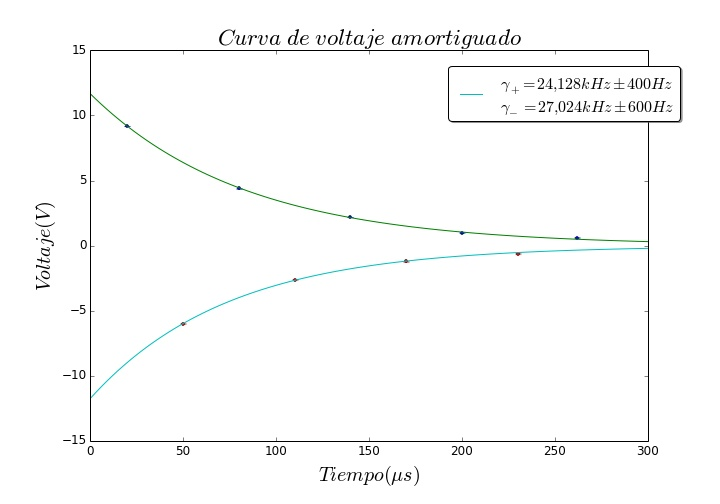
\includegraphics[width=0.45\textwidth]{amortiguado}
\label{fig:amortiguado}
\end{figure}

En este experimento volvimos a obtener un valor para $\gamma$ 2 ordenes de magnitud desfasado del valor te\'orico dado por la inductancia. Dado que el experimento es en principio diferente, as\'i como lo fue el m\'etodo de ajuste, tenemos evidencia fuerte para afirmar que la resistencia del inductor no era la \'unica resistencia que estaba presente en el circuito RLC armado. Las otras resistencias provienen de cada uno de los aparatos electr\'onicos utilizados y pueden haber fuentes grandes de resistencia en el \'oxido por edad y uso de algunos contactos en la protoboard, los cables, y los elementos LC, entre otros. Debido a la simplicidad de la funci\'on ajustada, y lo directo de la medida, podemos confiar m\'as en este valor para $\gamma$. Sin embargo, dado que descubrimos que estamos subestimando la resistencia total del circuito no podemos arrojar un porcentaje de error con respecto al valor te\'orico.

\subsection{\label{sec:level2}Curvas de Lissajous}
Para este montaje tomamos la misma amplitud para cada generador y variamos sus frecuencias y desfases para producir diferentes curvas de Lissajous. El voltaje $V_{pp}$ leido por el osciloscopio fue constante de $205V$. A continuación presentaremos tres imágenes que comparan curvas de Lissajous para una misma razón de frecuencias y distintos desfases. Cabe resaltar que tomamos fotografías únicamente para 2 desfases por cada razón de frecuencias, ya que los generadores se desfasaban naturalmente al cambiar de frecuencia y calibrarlos consumía bastante tiempo.\\

\begin{figure}[h!]
\caption{ Curvas de Lissajous. Razón 1:1, desfases ($\frac{\pi}{4}$,0) }
\centering
\includegraphics[width=0.45\textwidth]{1}
\label{fig:amortiguado}
\end{figure}

\begin{figure}[h!]
\caption{ Curvas de Lissajous. Razón 1:2, desfases (0,$\frac{\pi}{4}$) }
\centering
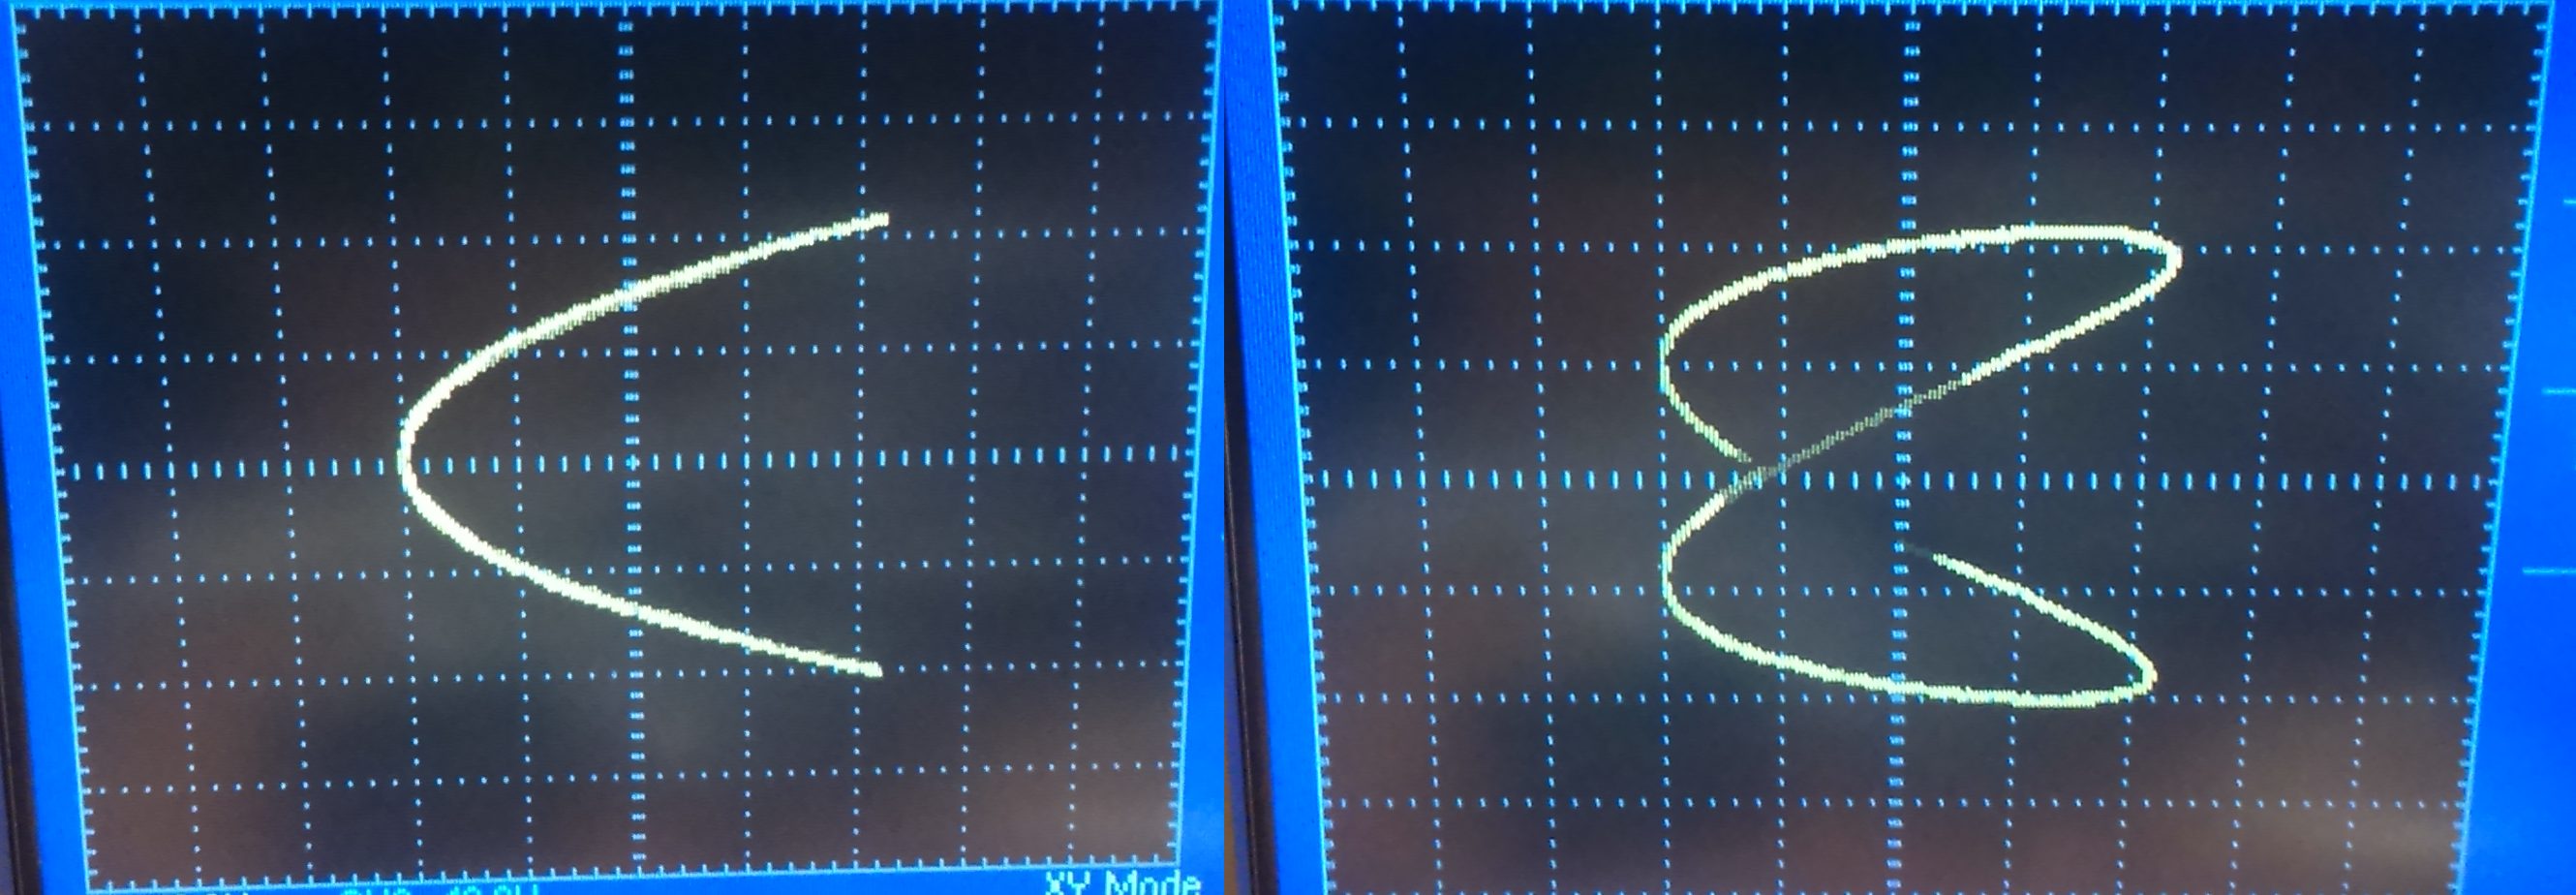
\includegraphics[width=0.45\textwidth]{2}
\label{fig:amortiguado}
\end{figure}

\begin{figure}[h!]
\caption{ Curvas de Lissajous. Razón 1:3, desfases (0,$\frac{\pi}{4}$) }
\centering
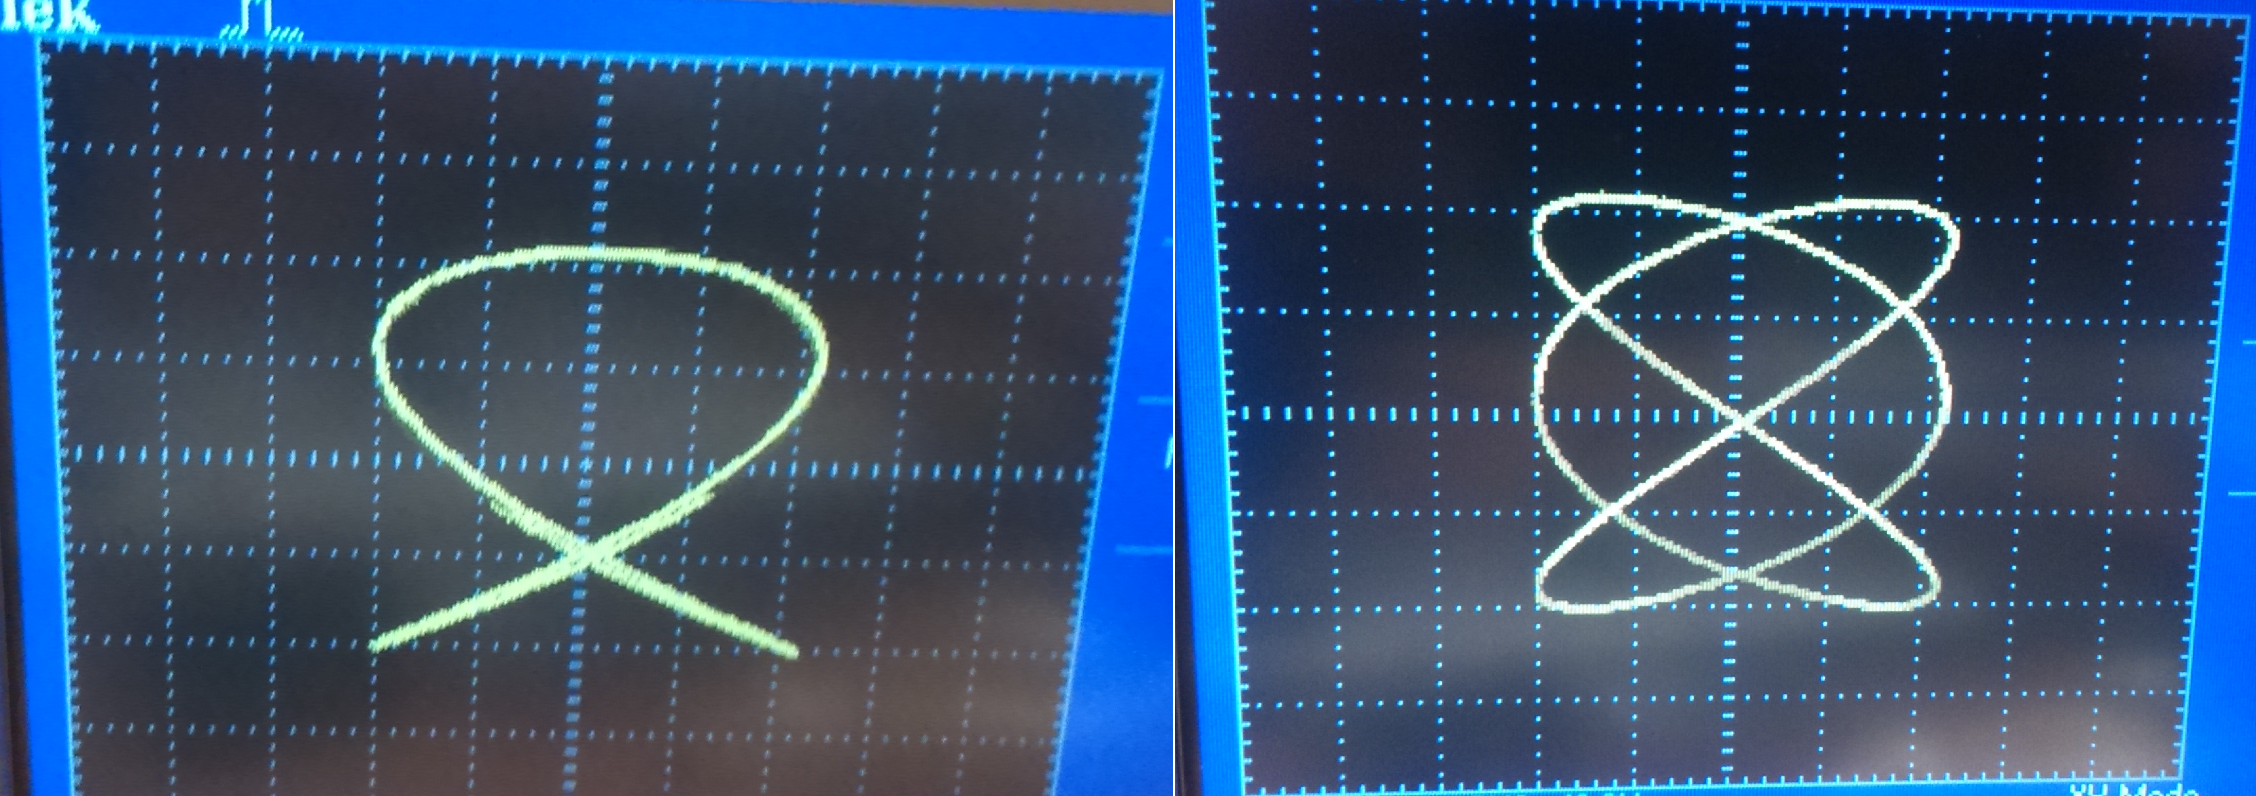
\includegraphics[width=0.45\textwidth]{3}
\label{fig:amortiguado}
\end{figure}

Al cambiar contínuamente la frecuencia, la imagen mostrada en el osciloscopio daba la impresión de estar rotando. Por otra parte, de estas figuras es importante notar que todas son cerradas. Esto era de esperarse ya que las frecuencias escogidas fueron tales que formaran racionales simples como 1/2 o 1/3 o 1. Esto nos indica también que la precisión con la que se generan las frecuencias es bastante grande como ya habíamos descrito. En caso de que dicha precisión no fuera tan buena, habríamos observado curvas de Lissajous muy dinámicas en la pantalla.\\


\section{\label{sec:level1}Conclusiones}
 \ \\


\begin{thebibliography}{99} 
\bibitem{ondas} A.P. French,{\it vibraciones y ondas}{Editorial Reverté s.a.,1971}, and references.\\ 
\bibitem{guia} Universidad de los Andes,{\it Guía 1 Osciloscopio}{2015}, and references.\\ \end{thebibliography}




\end{document}
%
% ****** End of file apssamp.tex ******
